% =====================================================================
%  Presentación (15 min): Redes neuronales difractivas en el visible
%  Compilar: latexmk -pdf presentacion.tex
% =====================================================================
\documentclass[aspectratio=169,10pt]{beamer}

\usepackage[T1]{fontenc}
\usepackage[utf8]{inputenc}
\usepackage[spanish,es-noshorthands,es-nodecimaldot]{babel}
\usepackage{lmodern}
\usepackage[final]{microtype}

\usepackage{amsmath,amssymb,mathtools,bm}
\usepackage{siunitx}
\sisetup{output-decimal-marker={.},group-separator={\,},per-mode=symbol,
         range-phrase={--},list-final-separator={ y }}

\usepackage{graphicx}
\graphicspath{{../tesina/figuras/}}
\usepackage{booktabs}
\usepackage{tikz}
\usetikzlibrary{calc,arrows.meta,decorations.pathreplacing,patterns,positioning}
\usepackage{pgfplots}
\pgfplotsset{compat=1.18}
\usepgfplotslibrary{fillbetween}
\usepackage[most]{tcolorbox}

% --- Paleta institucional (idéntica a la tesina) ----------------------
\definecolor{udlap}{HTML}{F37B20}
\definecolor{udlaposcuro}{HTML}{9A4A0E}
\definecolor{udlapclaro}{HTML}{FDEBDD}
\definecolor{gris}{HTML}{5E5E5E}
\definecolor{azulfig}{HTML}{2C6FB7}
\definecolor{azulclaro}{HTML}{EAF2FB}

% --- Operadores y macros ----------------------------------------------
\newcommand{\dd}{\,\mathrm{d}}
\newcommand{\jj}{\mathrm{j}}
\newcommand{\FT}{\mathcal{F}}
\newcommand{\IFT}{\mathcal{F}^{-1}}
\newcommand{\rect}{\operatorname{rect}}
\newcommand{\sinc}{\operatorname{sinc}}
\newcommand{\Real}{\operatorname{Re}}
\newcommand{\Imag}{\operatorname{Im}}
\newcommand{\Dmin}{D_{\min}}
\newcommand{\flim}{f_{\lim}}
\DeclareMathOperator*{\argmax}{arg\,max}

\newcommand{\placa}[3]{%
  \draw[#3] ($(#1,0)+(-0.22,-1.05)$) -- ($(#1,0)+(0.22,-0.68)$) -- ($(#1,0)+(0.22,1.18)$)
           -- ($(#1,0)+(-0.22,0.82)$) -- cycle;
  \node[font=\tiny,below] at ($(#1,0)+(0,-1.08)$) {#2};}

% --- Configuración visual de Beamer -----------------------------------
\usetheme{default}
\usecolortheme{default}
\setbeamertemplate{navigation symbols}{}
\setbeamercolor{structure}{fg=udlaposcuro}
\setbeamercolor{frametitle}{fg=udlaposcuro,bg=white}
\setbeamercolor{normal text}{fg=black!88,bg=white}
\setbeamercolor{itemize item}{fg=udlap}
\setbeamercolor{itemize subitem}{fg=azulfig}
\setbeamerfont{frametitle}{size=\large,series=\bfseries}
\setbeamerfont{framesubtitle}{size=\footnotesize,series=\normalfont}

\setbeamertemplate{frametitle}{%
  \vspace*{0.16cm}
  \begin{minipage}{\textwidth}
    {\usebeamerfont{frametitle}\usebeamercolor[fg]{frametitle}\insertframetitle\par}
    \ifx\insertframesubtitle\@empty\else
      {\vspace{1pt}\usebeamerfont{framesubtitle}\color{gris}\insertframesubtitle\par}
    \fi
    \vspace{2.5pt}
    {\color{udlap}\hrule height 1.1pt}
  \end{minipage}
  \vspace*{-0.18cm}
}

\setbeamertemplate{footline}{%
  \ifnum\theframenumber>1
  \leavevmode%
  \hbox{%
    \begin{beamercolorbox}[wd=.75\paperwidth,ht=2.1ex,dp=0.9ex,leftskip=0.45cm]{author in head/foot}%
      \color{gris}\scriptsize Redes neuronales difractivas en el visible \;|\; Proyecto Final de Óptica
    \end{beamercolorbox}%
    \begin{beamercolorbox}[wd=.25\paperwidth,ht=2.1ex,dp=0.9ex,rightskip=0.45cm,right]{date in head/foot}%
      \color{udlaposcuro}\scriptsize\bfseries \insertframenumber\,/\,\inserttotalframenumber
    \end{beamercolorbox}%
  }%
  \vspace{1pt}
  {\color{udlap}\hrule height 2.0pt}
  \fi
}

% --- Cajas estilizadas ------------------------------------------------
\newtcolorbox{caja}[2][udlaposcuro]{%
  colback=white,colframe=#1,boxrule=0.7pt,arc=2pt,
  left=5pt,right=5pt,top=3pt,bottom=3pt,
  fonttitle=\bfseries\footnotesize,title={#2},
  coltitle=white,colbacktitle=#1}

\newtcolorbox{destacado}[1][udlap]{%
  colback=udlapclaro,colframe=#1,boxrule=0.7pt,arc=2pt,
  left=5pt,right=5pt,top=3pt,bottom=3pt}

\newtcolorbox{azulbox}[1]{%
  colback=azulclaro,colframe=azulfig,boxrule=0.7pt,arc=2pt,
  left=5pt,right=5pt,top=3pt,bottom=3pt,
  fonttitle=\bfseries\footnotesize,title={#1},
  coltitle=white,colbacktitle=azulfig}

% --- Metadatos --------------------------------------------------------
\title{Redes neuronales difractivas en el visible}
\subtitle{Fundamentos de difracción escalar, criterio de conectividad y reproducción numérica de Chen et al.\ (2021)}
\author{Alonso Hernández Hernández y Ángel Gabriel Munguía Velázquez}
\institute{Universidad de las Américas Puebla — Proyecto Final de Óptica}
\date{San Andrés Cholula, Puebla, 2026}

\begin{document}

% =====================================================================
%  DIAPOSITIVA 1: PORTADA
% =====================================================================
\begin{frame}[plain]
\begin{tikzpicture}[remember picture,overlay]
  \coordinate (NW) at (current page.north west);
  \coordinate (SE) at (current page.south east);
  % Marco geométrico sutil (beamer 16:9 mide 16cm x 9cm)
  \draw[udlap!45,line width=0.6pt]
    ($(NW)+(0.6,-0.5)$) -- ($(NW)+(15.4,-0.5)$) -- ($(NW)+(14.7,-8.4)$)
    -- ($(NW)+(0.6,-8.2)$) -- cycle;
  % Arcos de difracción decorativos
  \foreach \r in {1,...,8}{
    \draw[udlap!18,line width=0.7pt] ($(NW)+(0.6,-8.2)$) ++(0:\r*0.38) arc (0:65:\r*0.38);
  }
  % Franja inferior
  \fill[udlap] (current page.south west) rectangle ($(SE)+(0,0.20)$);
  % Logo
  \node[anchor=north west,inner sep=0pt] at ($(NW)+(1.05,-0.78)$)
    {
\includegraphics[width=1.55cm]{logo_udlap.png}};
  \node[anchor=west,align=left] at ($(NW)+(2.85,-1.55)$)
    {\sffamily\small\bfseries\color{udlaposcuro}Universidad de las Américas Puebla\\[-1pt]
     \footnotesize\mdseries\color{gris}Curso de Óptica \;\textbullet\; Aplicaciones de la difracción};
  % Título
  \node[anchor=north west,text width=13.0cm,align=left] at ($(NW)+(1.15,-2.75)$) {%
    {\sffamily\footnotesize\bfseries\color{udlap} PROYECTO FINAL DE ÓPTICA \;|\; PRESENTACIÓN (15 MIN)\par}
    \vspace{5pt}
    {\sffamily\fontsize{21}{25}\selectfont\bfseries\color{black!90} Redes neuronales difractivas en el visible\par}
    \vspace{6pt}
    {\color{udlap}\rule{2.8cm}{2pt}\par}
    \vspace{6pt}
    {\sffamily\normalsize\color{gris} Fundamentos de difracción escalar, criterio de conectividad y reproducción numérica de Chen et al.\ (2021)\par}
  };
  % Pie de portada
  \node[anchor=north west,text width=13.0cm,align=left] at ($(NW)+(1.15,-6.45)$) {%
    \sffamily\small
    \textbf{Presentan:} Alonso Hernández Hernández y Ángel Gabriel Munguía Velázquez\\[3pt]
    \textbf{Profesor:} Dr.\ Wanderson Maia Pimienta \quad\textbullet\quad \textbf{Fecha:} 2026
  };
\end{tikzpicture}
\end{frame}

% =====================================================================
%  DIAPOSITIVA 2: DESCRIPCIÓN DEL SISTEMA ÓPTICO
% =====================================================================
\begin{frame}{Descripción del sistema: del régimen terahertz al visible}
\framesubtitle{La difracción realiza transformadas lineales en paralelo a la velocidad de la luz}
\begin{columns}[T,onlytextwidth]
  \begin{column}{0.44\textwidth}
    \footnotesize
    \begin{itemize}\setlength\itemsep{2.5pt}
      \item \textbf{Idea central (Goodman, 2005):} la propagación libre y las máscaras ópticas ejecutan convoluciones y transformadas de Fourier \textbf{sin gasto energético} adicional al haz.
      \item \textbf{D\textsuperscript{2}NN (Lin et al., 2018):} placas impresas en 3D en THz ($\lambda\approx\SI{0.75}{mm}$, neuronas de \SI{0.4}{mm}).
      \item \textbf{Salto al visible (Chen et al., 2021):} láser He--Ne ($\lambda=\SI{632.8}{nm}$) reduce el sistema en \textbf{3 órdenes de magnitud}, con neuronas litográficas de \SI{4}{\micro m}.
    \end{itemize}
    \vspace{2pt}
    \begin{destacado}
      \footnotesize\textbf{Hilo conductor:} al achicar las neuronas a \SI{4}{\micro m}, el cono cae de $\sim\ang{70}$ a $\ang{4.54}$. \emph{¿Cómo se fabrican estas placas y qué ecuaciones rigen la propagación y la separación mínima $D$?}
    \end{destacado}
  \end{column}
  \begin{column}{0.54\textwidth}
    \centering
    \begin{tikzpicture}[x=0.43cm,y=0.56cm,>={Stealth[length=1.6mm]},
      capa/.style={fill=udlap!25,draw=udlaposcuro,thick},
      plano/.style={fill=gray!12,draw=gray!70,thick}]
      \fill[red!12] (0.9,-0.22) -- (2.1,-0.85) -- (12.4,-0.85) -- (12.4,0.85) -- (2.1,0.85) -- cycle;
      \draw[fill=gray!65,rounded corners=2pt] (-0.75,-0.32) rectangle (0.9,0.32);
      \node[font=\tiny,white] at (0.07,0) {He--Ne};
      \node[font=\tiny,below] at (0.07,-0.35) {\SI{632.8}{nm}};
      \draw[thick,azulfig] (1.5,0) ellipse (0.06 and 0.42);
      \draw[very thick] (1.85,0.48) -- (1.85,0.06) (1.85,-0.06) -- (1.85,-0.48);
      \draw[thick,azulfig] (2.35,0) ellipse (0.10 and 0.95);
      \placa{3.35}{ent.}{plano}
      \node at (3.35,0.05) {\tiny\bfseries 3};
      \foreach \l/\x in {1/4.75,2/6.15,3/7.55,4/8.95,5/10.35} {\placa{\x}{$L_{\l}$}{capa}}
      \placa{11.85}{sal.}{plano}
      \foreach \yy in {-0.5,0,0.5} \draw[fill=white,draw=red!70!black] ($(11.85,\yy)+(-0.06,-0.08)$) rectangle ($(11.85,\yy)+(0.08,0.1)$);
      \draw[<->] (4.75,1.45) -- (6.15,1.45) node[midway,above,font=\tiny] {$D\approx\SI{5}{cm}$};
      \draw[decorate,decoration={brace,amplitude=3pt,mirror}] (4.5,-1.55) -- (10.6,-1.55)
         node[midway,below=3pt,font=\tiny] {5 capas de $1000\times1000$ neuronas ($d_f=\SI{4}{\micro m}$)};
      \draw[->,thick] (12.4,0) -- (13.0,0) node[right,font=\tiny] {$\argmax_k E_k$};
    \end{tikzpicture}
    \vspace{4pt}
    {\tiny\setlength{\tabcolsep}{4pt}
    \begin{tabular}{@{}ll@{}}
      \toprule
      Parámetro (Chen et al., 2021) & Valor \\
      \midrule
      Longitud de onda / capa & $\lambda=\SI{632.8}{nm}$,\; $w=\SI{4}{mm}$ ($1000^2$) \\
      Clases / entrenamiento & 11 (0--9 y ``X''),\; 80\,000 imgs., 20 épocas \\
      Modulación por neurona & Solo fase: $t^l_i=e^{\jj\Phi^l_i}$,\; $\Phi^l_i\in[0,\pi]$ \\
      \bottomrule
    \end{tabular}}
  \end{column}
\end{columns}
\end{frame}

% =====================================================================
%  DIAPOSITIVA 3: PROCESO DE FABRICACIÓN EN LABORATORIO (CHEN ET AL.)
% =====================================================================
\begin{frame}{Proceso de fabricación en laboratorio (Chen et al., 2021)}
\framesubtitle{Fotolitografía láser para objetos de entrada y grabado multinivel en obleas de $\mathrm{SiO_2}$}
\begin{columns}[T,onlytextwidth]
  \begin{column}{0.48\textwidth}
    \begin{azulbox}{1. Objetos de entrada (dígitos transmisivos)}
      \scriptsize
      \begin{itemize}\setlength\itemsep{2.5pt}
        \item \textbf{Preparación del sustrato:} vidrio de sosa (\emph{soda glass}) limpio con acetona y alcohol isopropílico.
        \item \textbf{Recubrimiento metálico:} película opaca de cromo ($\mathrm{Cr}$) por evaporación por haz de electrones.
        \item \textbf{Fotolitografía láser:} fotorresina positiva por rotación (\emph{spin-coating}), horneado previo y \textbf{Escritura Directa por Láser (LDW)} con la silueta exacta del dígito.
        \item \textbf{Grabado y limpieza (\emph{etching}):} revelado, mordiente de $\mathrm{Cr}$ en zonas expuestas y retiro final de fotorresina.
      \end{itemize}
    \end{azulbox}
  \end{column}
  \begin{column}{0.50\textwidth}
    \begin{caja}{2. Capas difractivas (la red $\text{D}^2\text{NN}$)}
      \scriptsize
      \begin{itemize}\setlength\itemsep{2.5pt}
        \item \textbf{Preparación del sustrato:} obleas de dióxido de silicio ($\mathrm{SiO_2}$) tratadas con hexametildisilazano (HMDS) para adherir la fotorresina.
        \item \textbf{Transferencia del diseño:} recubrimiento con fotorresina, exposición con el mapa de fases y revelado.
        \item \textbf{Grabado del relieve:} tratamiento con plasma de $\mathrm{O_2}$ y \textbf{grabado en seco por descarga de bucle neutro magnético} (\emph{NLD etching}) con precisión nanométrica.
        \item \textbf{Proceso iterativo multinivel:} repetición alineada ($s=3$ ciclos) para tallar $2^3=8$ niveles de relieve ($\Delta h_\pi=\SI{692}{nm}$).
      \end{itemize}
    \end{caja}
  \end{column}
\end{columns}
\end{frame}

% =====================================================================
%  DIAPOSITIVA 4: RAYLEIGH-SOMMERFELD Y MODULACIÓN DE FASE
% =====================================================================
\begin{frame}{Fundamento I: Huygens--Fresnel como sinapsis y relieve de fase}
\framesubtitle{Cada neurona emite una onda esférica secundaria modulada en retardo de fase}
\begin{columns}[T,onlytextwidth]
  \begin{column}{0.52\textwidth}
    \small\textbf{Integral de Rayleigh--Sommerfeld (1.\textsuperscript{a} especie):}
    {\footnotesize
    \[
      U(x,y,z)=\iint_{-\infty}^{\infty} U(x',y',0)\,h(x-x',y-y',z)\dd x'\dd y'
    \]
    \[
      h(x,y,z)=\frac{z}{2\pi r^2}\!\left(\frac{1}{r}-\jj k\right)\!e^{\jj kr}
      \;\xrightarrow{r\gg\lambda}\;
      \frac{1}{\jj\lambda}\underbrace{\frac{z}{r}}_{\cos\theta}\frac{e^{\jj kr}}{r}
    \]}
    \vspace{-4pt}
    \begin{center}
    \begin{tikzpicture}[scale=0.56,>={Stealth[length=1.8mm]}]
      \fill[gray!15] (0,-2.0) rectangle (0.18,2.0);
      \draw[thick] (0.18,-2.0) -- (0.18,2.0);
      \node[above,font=\scriptsize] at (0.1,2.0) {$z=0$};
      \foreach \x in {-1.8,-1.35,-0.9} \draw[azulfig!70,thick] (\x,-1.7) -- (\x,1.7);
      \foreach \y in {-1.2,-0.6,0,0.6,1.2}{
         \fill[udlap] (0.18,\y) circle (1.5pt);
         \foreach \r in {0.42,0.84,1.26}
            \draw[udlap!75] ($(0.18,\y)+(-75:\r)$) arc (-75:75:\r);
      }
      \draw[udlaposcuro,very thick,dashed] (1.44,-1.7) -- (1.44,1.7);
      \coordinate (P) at (4.8,0.8);
      \fill (P) circle (1.8pt) node[right,font=\scriptsize] {$P(x,y,z)$};
      \draw[->,gray] (0.18,-0.6) -- (P) node[midway,below,sloped,font=\scriptsize] {$r$};
      \draw[gray,dashed] (0.18,-0.6) -- (4.8,-0.6);
      \node[gray,font=\scriptsize] at (1.7,-0.35) {$\theta$};
      \draw[->] (0.18,-2.25) -- (5.4,-2.25) node[right,font=\scriptsize] {$z$};
    \end{tikzpicture}
    \end{center}
  \end{column}
  \begin{column}{0.46\textwidth}
    \begin{caja}{De la fase a la altura grabada en sílice fundida}
      \scriptsize
      Cada neurona impone una fase $\Phi\in[0,\pi]$ mediante un escalón de relieve $\Delta h$ en vidrio ($n=1.4570$, $\Delta n=0.457$):
      \[
        \Phi=\frac{2\pi}{\lambda}\Delta n\,\Delta h
        \;\Longrightarrow\;
        \Delta h_\pi=\frac{\lambda}{2\Delta n}=\SI{692}{nm}.
      \]
      Con $s=3$ pasos litográficos ($2^3=8$ niveles), cada escalón mide \SI{98.9}{nm}.
    \end{caja}
    \vspace{5pt}
    \begin{azulbox}{Pérdidas de Fresnel ignoradas en el artículo}
      \scriptsize
      En cada interfaz aire--vidrio la reflectancia a incidencia normal es
      $R=\left(\frac{n-1}{n+1}\right)^2=3.46\%$.\\[3pt]
      En 5 capas (10 interfaces), la transmisión total es $(1-R)^{10}\approx 70\%$ (reduce la señal absoluta, pero no cambia la razón entre detectores).
    \end{azulbox}
  \end{column}
\end{columns}
\end{frame}

% =====================================================================
%  DIAPOSITIVA 5: ESPECTRO ANGULAR, FUNCIÓN H(u,v;z) Y FALLA DE FRESNEL
% =====================================================================
\begin{frame}{Fundamento II: Espectro angular y por qué falla Fresnel}
\framesubtitle{De la ecuación de Helmholtz al propagador exacto en el dominio de Fourier}
\begin{columns}[T,onlytextwidth]
  \begin{column}{0.51\textwidth}
    \footnotesize
    \textbf{Ecuación de Helmholtz:} $(\nabla^2+k^2)U(\bm r)=0$.
    Con $\rho^2=u^2+v^2$:
    \[
      A(u,v;z)=A(u,v;0)\,\exp\!\left[\jj kz\sqrt{1-\lambda^2\rho^2}\right]
    \]
    \begin{destacado}
      \scriptsize\vspace{-3pt}
      \[
        H(u,v;z)=
        \begin{cases}
          \exp\!\left[\jj kz\sqrt{1-\lambda^2\rho^2}\right], & \rho^2\le 1/\lambda^2\\
          \exp\!\left[-2\pi z\sqrt{\rho^2-1/\lambda^2}\right], & \rho^2> 1/\lambda^2
        \end{cases}
      \]
      \vspace{-4pt}
      \[
        U(x,y,z)=\IFT\Bigl\{\FT\{U(x,y,0)\}\cdot H(u,v;z)\Bigr\}
      \]
    \end{destacado}
    \vspace{1pt}
    {\scriptsize\color{gris} Nota: Chen et al.\ (Ecs.\ 4--5) escriben $W^{l+1}\cdot H$ en lugar de operar en Fourier. La red es \textbf{lineal en el campo}; la única no linealidad es $|Y^{\text{sal}}|^2$.}
  \end{column}
  \begin{column}{0.47\textwidth}
    \begin{caja}{¿Sirve la aproximación de Fraunhofer?}
      \scriptsize
      Exige $z\gg ka^2/2=\pi a^2/\lambda\approx\SI{19.9}{m}$ ($a=\SI{2}{mm}$). Con $D=\SI{5}{cm}$, el número de Fresnel de la capa es:
      \[
        N_F=\frac{a^2}{\lambda D}=\frac{(\SI{2}{mm})^2}{\SI{632.8}{nm}\times\SI{5}{cm}}\approx\mathbf{126}
      \]
      $\implies$ opera profundamente en \textbf{campo cercano}.
    \end{caja}
    \vspace{3pt}
    \begin{azulbox}{¿Sirve la aproximación de Fresnel?}
      \scriptsize
      Al expandir $\sqrt{1-s}=1-\frac{s}{2}-\frac{s^2}{8}-\cdots$ ($s=\lambda^2\rho^2$), exige que la fase despreciada cumpla
      $\frac{1}{4}\pi z\lambda^3\rho^4\ll 1$.\\[2pt]
      Para $\rho=1/(2d_f)$ ($d_f=\SI{4}{\micro m}$): \textbf{\SI{2.4}{rad}} en ejes y \textbf{\SI{9.7}{rad}} en diagonal $\implies$ \textbf{Fresnel no es válida}; se requiere $H$ exacta.
    \end{azulbox}
  \end{column}
\end{columns}
\end{frame}

% =====================================================================
%  DIAPOSITIVA 6: DIFRACCIÓN DE UNA NEURONA Y FACTOR 2
% =====================================================================
\begin{frame}{Difracción de una neurona: el origen del factor 2 en $\varphi_{\max}$}
\framesubtitle{El límite $\sin\varphi_{\max}=\lambda/(2d_f)$ no es el primer cero de la sinc, sino Nyquist}
\begin{columns}[T,onlytextwidth]
  \begin{column}{0.51\textwidth}
    \centering
    \begin{tikzpicture}
    \begin{axis}[width=1.02\textwidth,height=4.9cm,
      xlabel={$d_f\,u=d_f\sin\theta/\lambda$}, ylabel={$\sinc^2(d_fu)$},
      xmin=-2.4,xmax=2.4,ymin=0,ymax=1.12,samples=320,domain=-2.4:2.4,
      xtick={-2,-1,-0.5,0,0.5,1,2},
      xticklabels={$-2$,$-1$,$-\tfrac12$,$0$,$\tfrac12$,$1$,$2$},
      axis lines=left,grid=major,grid style={gray!20},
      label style={font=\footnotesize},tick label style={font=\scriptsize},
      legend style={at={(0.98,0.97)},anchor=north east,font=\scriptsize,draw=none,fill=white}]
      \addplot[name path=f,very thick,udlap] {x==0 ? 1 : (sin(deg(pi*x))/(pi*x))^2};
      \addlegendentry{intensidad de una neurona}
      \path[name path=axis] (axis cs:-0.5,0) -- (axis cs:0.5,0);
      \addplot[udlap!25] fill between[of=f and axis,soft clip={domain=-0.5:0.5}];
      \addlegendentry{Nyquist: 77.4\% energía (1D)}
      \draw[dashed,thick,azulfig] (axis cs:0.5,0) -- (axis cs:0.5,0.72);
      \node[anchor=west,font=\scriptsize,azulfig] at (axis cs:0.53,0.62) {$\sin\varphi_{\max}=\frac{\lambda}{2d_f}$};
      \draw[dashed,thick,gray] (axis cs:1,0) -- (axis cs:1,0.28)
         node[above,font=\scriptsize,align=center] {1.\textsuperscript{er} cero\\$\lambda/d_f$};
      \draw[dotted,thick] (axis cs:-2.4,0.405) -- (axis cs:0.5,0.405);
      \node[font=\scriptsize,anchor=south west] at (axis cs:-2.35,0.41) {$4/\pi^2\approx0.405$};
    \end{axis}
    \end{tikzpicture}
  \end{column}
  \begin{column}{0.47\textwidth}
    \footnotesize
    \begin{itemize}\setlength\itemsep{2.5pt}
      \item \textbf{Neurona aislada:} $\rect(x/d_f)$ tiene espectro $d_f\sinc(d_fu)$; su primer cero está en $\sin\theta=\lambda/d_f$.
      \item \textbf{Capa completa:} arreglo periódico con paso $d_f$:
      \[
        t(x)=\Bigl[\sum_i t_i\,\delta(x-i\,d_f)\Bigr]*\rect\!\left(\frac{x}{d_f}\right)
      \]
      \item \textbf{Teorema de muestreo (Shannon, 1949):} los pesos independientes $t_i=e^{\jj\Phi_i}$ sólo fijan frecuencias en $|u|\le \frac{1}{2d_f}$ (59.9\% energía 2D).
    \end{itemize}
    \vspace{2pt}
    \begin{destacado}
      \centering\footnotesize
      $\sin\varphi_{\max}=\lambda u_{\text{Nyq}}=\dfrac{\lambda}{2d_f}
      \;\Longrightarrow\;\varphi_{\max}=\mathbf{\ang{4.54}}$\\[2pt]
      {\scriptsize(vs.\ $\approx\ang{70}$ en THz; mantener $\ang{70}$ en visible exigiría $d_f\approx\SI{330}{nm}$).}
    \end{destacado}
  \end{column}
\end{columns}
\end{frame}

% =====================================================================
%  DIAPOSITIVA 7: CRITERIO DE CONECTIVIDAD Y NÚMERO DE FRESNEL
% =====================================================================
\begin{frame}{Criterio de conectividad ($\Dmin$) y número de Fresnel neuronal ($N_{F,n}$)}
\framesubtitle{Reducción adimensional en el régimen paraxial (Proposición 4.1)}
\begin{columns}[T,onlytextwidth]
  \begin{column}{0.49\textwidth}
    \centering
    \begin{tikzpicture}[x=0.44cm,y=0.42cm,>={Stealth[length=1.6mm]}]
      \def\D{6.4}\def\w{3.5}
      \fill[udlap!25] (-0.12,0) rectangle (0.12,\w);
      \fill[udlap!25] (\D-0.12,0) rectangle (\D+0.12,\w);
      \draw[udlaposcuro,thick] (-0.12,0) rectangle (0.12,\w);
      \draw[udlaposcuro,thick] (\D-0.12,0) rectangle (\D+0.12,\w);
      \foreach \i in {1,...,8} {\draw[udlaposcuro!55] (-0.12,\i*0.388) -- (0.12,\i*0.388);
                                \draw[udlaposcuro!55] (\D-0.12,\i*0.388) -- (\D+0.12,\i*0.388);}
      \node[above,font=\scriptsize] at (0,\w+0.05) {capa $l$};
      \node[above,font=\scriptsize] at (\D,\w+0.05) {capa $l+1$};
      \fill[udlaposcuro] (-0.12,0) rectangle (0.12,0.388);
      \fill[azulfig!12] (0.12,0.19) -- (\D-0.12,3.85) -- (\D-0.12,-3.45) -- cycle;
      \draw[azulfig,thick] (0.12,0.19) -- (\D-0.12,3.85);
      \draw[azulfig,thick] (0.12,0.19) -- (\D-0.12,-3.45);
      \draw[dashed,gray] (0.12,0.19) -- (\D+0.6,0.19);
      \draw[azulfig] (1.5,0.19) arc (0:30:1.38);
      \node[azulfig,font=\scriptsize] at (2.25,0.68) {$\varphi_{\max}$};
      \draw[<->,azulfig] (\D+0.3,0.19) -- (\D+0.3,3.85) node[midway,right,font=\tiny,align=left] {$R=$\\$D\tan\varphi_{\max}$};
      \draw[<->] (-0.4,0) -- (-0.4,\w) node[midway,left,font=\scriptsize] {$w$};
      \draw[<->] (0,-0.4) -- (\D,-0.4) node[midway,fill=white,font=\scriptsize] {$D$};
    \end{tikzpicture}
    \vspace{-4pt}
    {\scriptsize
    \[
      R\ge w \;\Longrightarrow\;
      \boxed{D\ge\Dmin\equiv\sqrt N\,d_f\sqrt{\frac{4d_f^2}{\lambda^2}-1}=\mathbf{\SI{50.4}{mm}}}
    \]}
    {\scriptsize Límite paraxial ($d_f\gg\lambda$): $\Dmin\approx 2\sqrt N\,d_f^2/\lambda$. El artículo usa $D\approx\SI{5}{cm}$.}
  \end{column}
  \begin{column}{0.49\textwidth}
    \begin{azulbox}{Proposición 4.1: invariancia por $N_{F,n}$}
      \scriptsize
      En Fresnel, con $u=m/(N_pd_f)$, el propagador se escribe:
      \[
        e^{-\jj\pi\lambda D(u^2+v^2)}
        =\exp\!\left[-\jj\pi\,\frac{m^2+m'^2}{N_{F,n}\,N_p^2}\right],
        \quad N_{F,n}\equiv\frac{d_f^2}{\lambda D}.
      \]
      Dos redes con iguales $\sqrt N$, $L$ y $N_{F,n}$ son \textbf{ópticamente equivalentes}, y
      \[
        \frac{D}{\Dmin}\approx\frac{1}{2\sqrt N\,N_{F,n}}.
      \]
    \end{azulbox}
    \vspace{2pt}
    \begin{caja}{Significado físico de $N_{F,n}$}
      \scriptsize
      $N_{F,n}$ cuenta cuántas zonas de Fresnel abarca una neurona desde la capa siguiente: si $N_{F,n}\gg 1$, la propagación es casi geométrica (cada neurona solo ilumina a su vecina); se exige $N_{F,n}\le 1/(2\sqrt N)$ para mezclar toda la capa.
    \end{caja}
  \end{column}
\end{columns}
\end{frame}

% =====================================================================
%  DIAPOSITIVA 8: DEL PERCEPTRÓN ELECTRÓNICO A LA RED DIFRACTIVA
% =====================================================================
\begin{frame}{Del perceptrón electrónico a la red neuronal difractiva ($\text{D}^2\text{NN}$)}
\framesubtitle{Cómo se traducen matrices y activaciones de silicio a difracción coherente en vidrio}
\begin{columns}[T,onlytextwidth]
  \begin{column}{0.45\textwidth}
    \begin{caja}{Perceptrón formal y red multicapa (MLP)}
      \scriptsize
      Una neurona pondera sus entradas y aplica una función no lineal:
      \[
        z=\mathbf{w}^\top\mathbf{x}+b,\qquad y=g(z),
      \]
      trazando un hiperplano separador que se ajusta por error: $w_i\leftarrow w_i-\eta(y-t)x_i$.\\[3pt]
      Apilar $L$ capas forma un MLP capaz de clasificar dígitos:
      \[
        \mathbf{a}^{[l]}=\sigma\!\left(\mathbf{W}^{[l]}\mathbf{a}^{[l-1]}+\mathbf{b}^{[l]}\right).
      \]
    \end{caja}
  \end{column}
  \begin{column}{0.53\textwidth}
    \begin{azulbox}{Correspondencia física MLP $\leftrightarrow$ $\text{D}^2\text{NN}$}
      \scriptsize\setlength{\tabcolsep}{3.5pt}
      \begin{tabular}{@{}lll@{}}
        \toprule
        Elemento & Red digital (MLP) & Red difractiva ($\text{D}^2\text{NN}$)\\
        \midrule
        Neurona & Activación $a_i^{[l]}$ & Píxel de vidrio ($\SI{4}{\micro m}$)\\
        Pesos & Matriz $\mathbf{W}^{[l]}$, sesgo $\mathbf{b}^{[l]}$ & Fase de transmisión $e^{\jj\Phi(x,y)}$\\
        Conexión & Producto $\mathbf{W}^{[l]}\mathbf{a}^{[l-1]}$ & Difracción Huygens--Fresnel\\
        No lin. & $\sigma(z)$ en cada capa & Solo detección $I=|U|^2$\\
        \bottomrule
      \end{tabular}\\[4pt]
      \textbf{Clave física:} la cascada óptica es \textbf{estrictamente lineal} en el campo eléctrico hasta los fotodetectores.
    \end{azulbox}
  \end{column}
\end{columns}
\end{frame}

% =====================================================================
%  DIAPOSITIVA 7: CONECTIVIDAD = MUESTREO Y VALIDACIÓN
% =====================================================================
\begin{frame}{Conectividad física $=$ muestreo numérico ($\Dmin = z_c$)}
\framesubtitle{Espectro angular de banda limitada (Matsushima \& Shimobaba, 2009) y validación}
\begin{columns}[T,onlytextwidth]
  \begin{column}{0.49\textwidth}
    \centering
    \begin{tikzpicture}[x=0.47cm,y=0.47cm,>={Stealth[length=1.6mm]}]
      \fill[gray!8] (0,0) rectangle (8,2.8);
      \draw[gray,thick,dashed] (0,0) rectangle (8,2.8);
      \node[gray,font=\tiny,rotate=90] at (0.9,1.4) {ceros};
      \node[gray,font=\tiny,rotate=90] at (7.1,1.9) {ceros};
      \fill[udlap!25] (2,0) rectangle (6,2.8);
      \draw[udlaposcuro,thick] (2,0) rectangle (6,2.8);
      \node[udlaposcuro,font=\scriptsize] at (4,2.45) {capa, $w=\sqrt N d_f$};
      \fill[udlaposcuro] (2.05,0.68) circle (1.6pt);
      \draw[->,very thick,azulfig] (2.05,0.68) -- (6.0,1.9) node[pos=0.52,above,sloped,font=\tiny] {$u\le \flim$};
      \draw[->,thick,red!70!black,dashed] (2.05,0.68) -- (8.0,1.12);
      \draw[<->] (2.05,-0.28) -- (6.0,-0.28) node[midway,below,font=\tiny] {$z\tan\theta\le w$};
      \draw[<->] (0,3.1) -- (8,3.1) node[midway,above,font=\tiny] {$N_p\Delta x=2w$ ($2\times$ relleno)};
    \end{tikzpicture}
    \vspace{2pt}
    \begin{destacado}
      \scriptsize
      \textbf{Proposición 5.1:} evitar el \emph{aliasing} de fase en $H$ exige $|u|\le \flim = \frac{1}{\lambda\sqrt{(2\Delta u\,z)^2+1}}$, que igualado a $\frac{1}{2\Delta x}$ define:
      \[
        z_c=\frac{N_p\Delta x}{2}\sqrt{\frac{4\Delta x^2}{\lambda^2}-1}
        \;\xrightarrow{\Delta x=d_f,\,N_p=2\sqrt N}\;
        \mathbf{z_c\equiv\Dmin}.
      \]
      Verificado en 15 pares $(\sqrt N, d_f/\lambda)$: $\flim(\Dmin)\cdot 2d_f = \mathbf{1.000000}$.
    \end{destacado}
  \end{column}
  \begin{column}{0.49\textwidth}
    \centering
    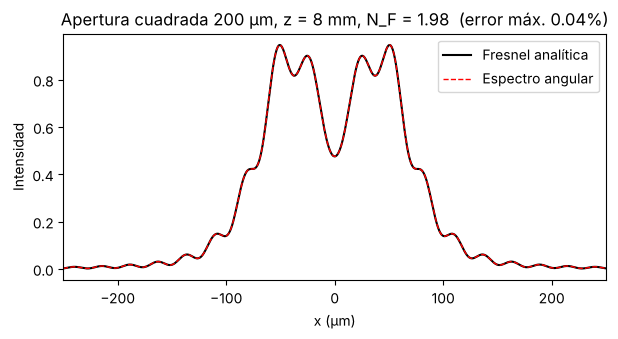
\includegraphics[width=0.73\textwidth]{b_apertura_cuadrada_fresnel.png}\\[2pt]
    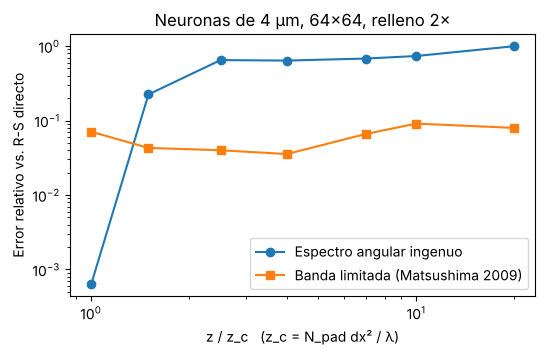
\includegraphics[width=0.71\textwidth]{c_aliasing_asm.png}\\[1pt]
    {\tiny Validación: \textbf{0.04\%} vs.\ Fresnel analítica; \textbf{3.6\%} vs.\ R--S circular ($z\ge\SI{0.3}{mm}$); \textbf{3.5--9.1\%} banda limitada vs.\ \textbf{22--99\%} ingenuo.}
  \end{column}
\end{columns}
\end{frame}

% =====================================================================
%  DIAPOSITIVA 8: RETROPROPAGACIÓN COMO HOLOGRAFÍA
% =====================================================================
\begin{frame}{Entrenamiento óptico: gradiente holográfico (Wirtinger)}
\framesubtitle{El error viaja hacia atrás en el tiempo con $H^*(u,v;D)=H(u,v;-D)$}
\centering
\begin{tikzpicture}[x=0.72cm,y=0.62cm,>={Stealth[length=1.6mm]},
   nodo/.style={draw,rounded corners=2pt,minimum width=0.95cm,minimum height=0.50cm,font=\scriptsize,fill=white},
   mascara/.style={nodo,fill=udlap!25,draw=udlaposcuro}]
  \node[nodo] (in) at (0,0) {$Y^{\text{ent}}$};
  \node[mascara] (t1) at (2.7,0) {$\circ\,t^1$};
  \node[mascara] (t2) at (5.4,0) {$\circ\,t^2$};
  \node (dots) at (7.3,0) {$\cdots$};
  \node[mascara] (tL) at (9.2,0) {$\circ\,t^L$};
  \node[nodo] (I) at (12.4,0) {$|\cdot|^2,\ \mathcal{L}$};
  \draw[->,thick] (in) -- node[above,font=\tiny]{$\mathcal{P}_D$ ($H$)} (t1);
  \draw[->,thick] (t1) -- node[above,font=\tiny]{$\mathcal{P}_D$} (t2);
  \draw[->,thick] (t2) -- (dots);
  \draw[->,thick] (dots) -- (tL);
  \draw[->,thick] (tL) -- node[above,font=\tiny]{$\mathcal{P}_D$} (I);

  \node[nodo,draw=azulfig] (g1) at (2.7,-2.05) {$G^{W,1}$};
  \node[nodo,draw=azulfig] (g2) at (5.4,-2.05) {$G^{W,2}$};
  \node (dots2) at (7.3,-2.05) {$\cdots$};
  \node[nodo,draw=azulfig] (gL) at (9.2,-2.05) {$G^{W,L}$};
  \node[nodo,draw=azulfig] (gs) at (12.4,-2.05) {$G^{\text{sal}}=c\,Y^{\text{sal}}$};
  \draw[->,thick,azulfig] (I) -- (gs);
  \draw[->,thick,azulfig] (gs) -- node[below=1pt,font=\tiny]{$\mathcal{P}_D^\dagger$ ($H^*$)} (gL);
  \draw[->,thick,azulfig] (gL) -- (dots2);
  \draw[->,thick,azulfig] (dots2) -- node[below=1pt,font=\tiny]{$\mathcal{T}^\dagger,\mathcal{P}_D^\dagger$} (g2);
  \draw[->,thick,azulfig] (g2) -- node[below=1pt,font=\tiny]{$\mathcal{T}^\dagger,\mathcal{P}_D^\dagger$} (g1);

  \foreach \a/\b in {t1/g1,t2/g2,tL/gL}{
     \draw[->,dashed,udlaposcuro] (\a) -- (\b);
     \node[font=\tiny,udlaposcuro,fill=white,inner sep=1pt] at ($(\a)!0.5!(\b)$) {$2\,\Imag\{G^{W}W^*\}$};}
  \node[font=\tiny,anchor=east] at (-0.95,0) {onda ($+D$)};
  \node[font=\tiny,anchor=west,azulfig] at (-0.85,-2.65) {onda de error ($-D$)};
\end{tikzpicture}
\vspace{4pt}
\begin{columns}[T,onlytextwidth]
  \begin{column}{0.46\textwidth}
    \begin{destacado}
      \scriptsize
      Si $G\equiv\partial\mathcal{L}/\partial Y^*$, el operador adjunto de $\mathcal{P}_D$ conjuga la función de transferencia ($\mathcal{P}_D^\dagger=\mathcal{P}_{-D}$) y en cada capa el gradiente es:
      \[
        \frac{\partial\mathcal{L}}{\partial\Phi_i^l}=2\,\Imag\!\left\{G_i^{W,l}\,(W_i^l)^*\right\}.
      \]
    \end{destacado}
  \end{column}
  \begin{column}{0.52\textwidth}
    \begin{caja}{Comprobación numérica (\texttt{07\_check\_gradient.py})}
      \scriptsize
      Red $32\times 32$, 5 capas, doble precisión (error relativo $\times 10^{-16}$):\\[2pt]
      \centering\scriptsize\setlength{\tabcolsep}{4pt}
      \begin{tabular}{@{}cccccc@{}}
        \toprule
        Capa 1 & Capa 2 & Capa 3 & Capa 4 & Capa 5 & Total\\
        \midrule
        4.90 & 5.31 & 5.10 & 4.79 & 3.43 & \textbf{4.49}\\
        \bottomrule
      \end{tabular}\\[2pt]
      \raggedright\scriptsize Acuerda con \texttt{autograd} al nivel del redondeo de máquina.
    \end{caja}
  \end{column}
\end{columns}
\end{frame}

% =====================================================================
%  DIAPOSITIVA 9: REPRODUCCIÓN DE LA FIG. 6 E INCONSISTENCIAS
% =====================================================================
\begin{frame}{Resultados I: Reproducción de la Fig.\ 6 e inconsistencias}
\framesubtitle{Red reducida de $80\times 80$ neuronas, 5 capas, 10 clases (MNIST)}
\begin{columns}[T,onlytextwidth]
  \begin{column}{0.50\textwidth}
    \centering
    {\tiny\setlength{\tabcolsep}{3.5pt}
    \begin{tabular}{@{}lccccc@{}}
      \toprule
      Caso & $d_f\,(\lambda)$ & $D\,(\lambda)$ & $D/\Dmin$ & Paper & Aquí \\
      \midrule
      1 & 0.53 & 15 & 1.01 & 90.0\% & \textbf{89.8\%} \\
      2 & 6 & $5.7\times10^3$ & 0.99 & 91.0\% & \textbf{89.0\%} \\
      3 (gráf.) & 6 & $2.4\times10^4$ & 4.18 & 91.2\% & 84.8\% \\
      3 (tabla) & 6 & $2.4\times10^3$ & 0.42 & 91.2\% & \textbf{91.2\%} \\
      4 & 12 & 15 & \num{6.5e-4} & ``$\sim$0.1'' & 14.4\% \\
      \bottomrule
    \end{tabular}}
    \vspace{2pt}
    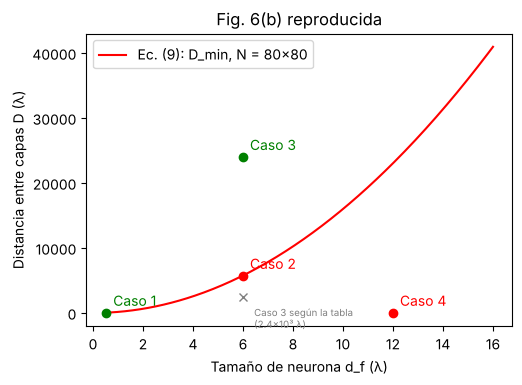
\includegraphics[width=0.53\textwidth]{e_fig6b_curva.png}
  \end{column}
  \begin{column}{0.48\textwidth}
    \centering
    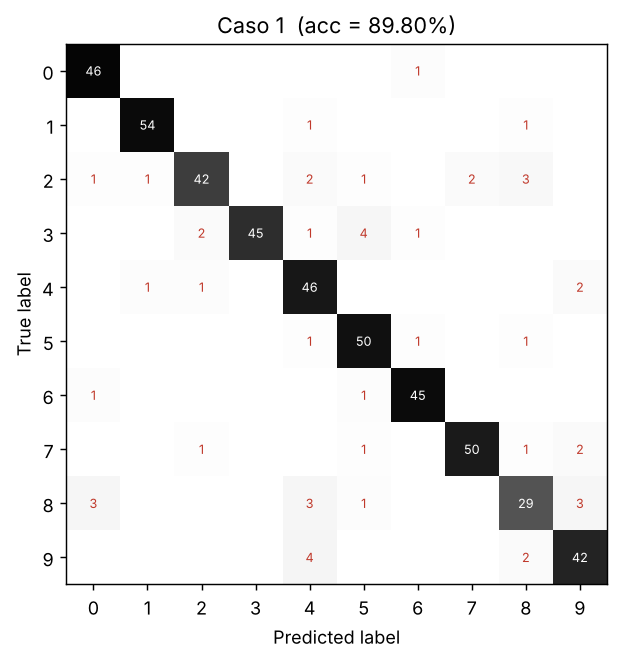
\includegraphics[width=0.31\textwidth]{confusion_caso1.png}\hspace{4pt}
    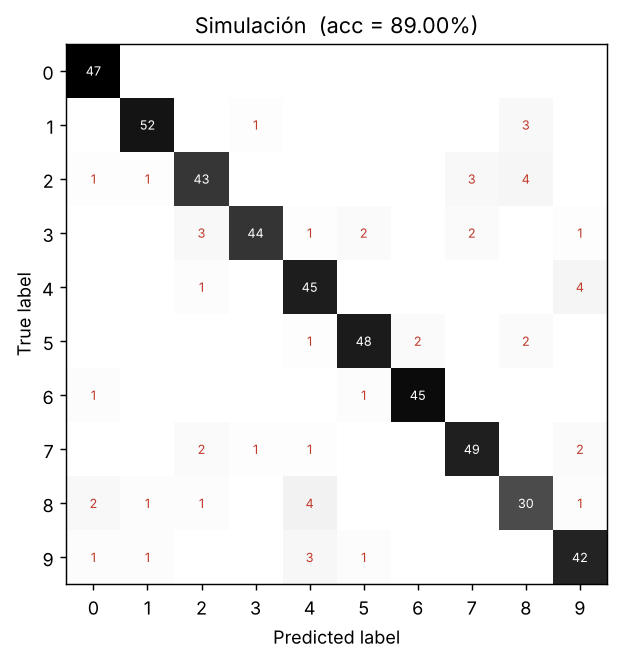
\includegraphics[width=0.31\textwidth]{confusion_caso2.png}\\[2pt]
    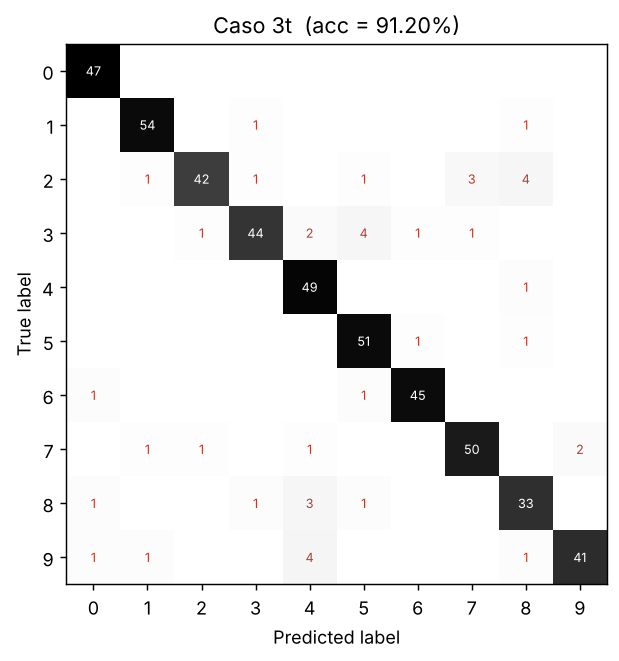
\includegraphics[width=0.31\textwidth]{confusion_caso3_tabla.png}\hspace{4pt}
    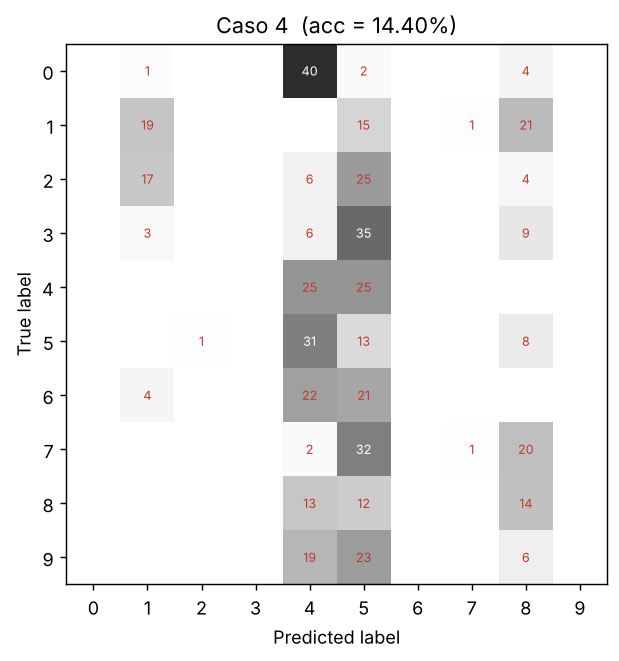
\includegraphics[width=0.31\textwidth]{confusion_caso4.png}
    \vspace{2pt}
    \begin{azulbox}{Hallazgos críticos en el artículo}
      \scriptsize
      \textbf{1. Caso 3:} con $D$ de la tabla ($0.42\,\Dmin$) reproducimos \textbf{91.2\%} exacto; en la gráfica está $10\times$ arriba ($4.18\,\Dmin$), donde perdemos luz por borde (84.8\%).\\
      \textbf{2. Caso 4:} ``$\sim 0.1$'' es fracción ($\approx$ azar 10\%). Con $R\approx 0.6\lambda < d_f$ no hay mezcla espacial.
    \end{azulbox}
  \end{column}
\end{columns}
\end{frame}

% =====================================================================
%  DIAPOSITIVA 10: BARRIDO DE CONECTIVIDAD
% =====================================================================
\begin{frame}{Resultados II: Barrido de conectividad y capas ($L=1,3,5,8$)}
\framesubtitle{Colapso universal por $N_{F,n}$ (20 épocas) y verificación de la conectividad acumulada}
\begin{columns}[T,onlytextwidth]
  \begin{column}{0.57\textwidth}
    \centering
    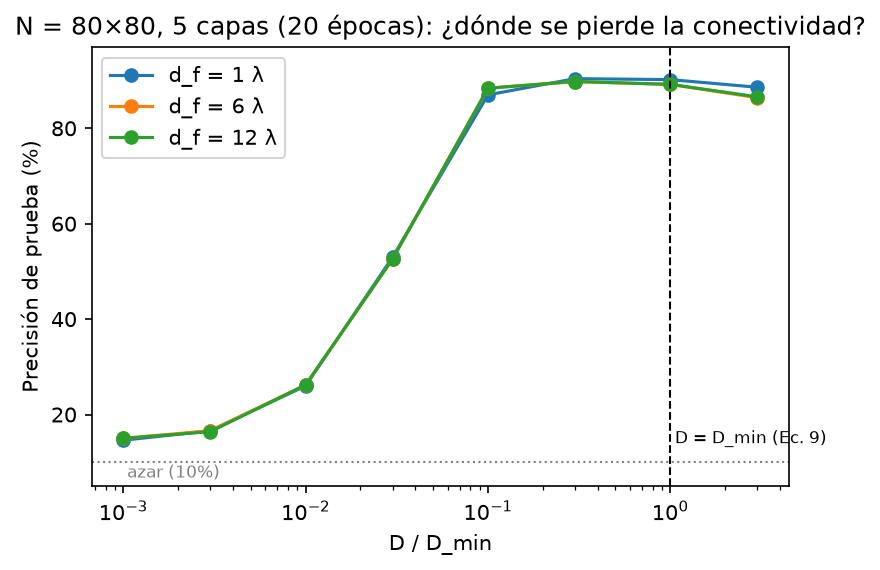
\includegraphics[width=0.49\textwidth]{sweep.png}\hfill
    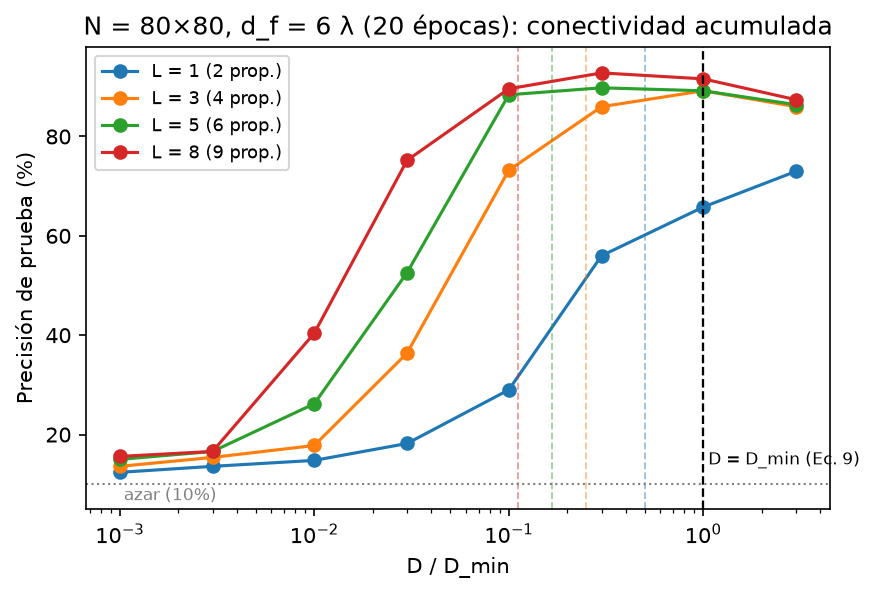
\includegraphics[width=0.49\textwidth]{sweep_layers.png}\\[2pt]
    {\tiny\setlength{\tabcolsep}{1.7pt}
    \begin{tabular}{@{}lccccccc@{}}
      \toprule
      $D/\Dmin$ & $10^{-3}$ & $0.01$ & $0.03$ & $0.1$ & $0.3$ & $1$ & $3$ \\
      \midrule
      $1\lambda$ ($L{=}5$)  & 14.6 & 26.0 & 53.0 & 87.0 & \textbf{90.4} & 90.2 & 88.6 \\
      $6\lambda$ ($L{=}5$)  & 15.0 & 26.2 & 52.6 & 88.4 & \textbf{89.8} & 89.2 & 86.4 \\
      $12\lambda$ ($L{=}5$) & 15.0 & 26.2 & 52.6 & 88.4 & \textbf{89.8} & 89.2 & 86.6 \\
      \midrule
      $L{=}1/8$ ($6\lambda$) & 12.4/15.6 & 14.8/40.4 & 18.2/75.2 & 29.0/89.6 & 56.0/\textbf{92.8} & 65.8/91.6 & 73.0/87.4 \\
      \bottomrule
    \end{tabular}}
  \end{column}
  \begin{column}{0.41\textwidth}
    \begin{caja}{1. $D/\Dmin$ es la variable universal}
      \scriptsize
      Para $d_f=6\lambda$ y $12\lambda$ las curvas casi coinciden (Proposición 4.1: mismo $N_{F,n}$). Con $1\lambda$ difiere $<1$ punto en la transición.
    \end{caja}
    \vspace{3pt}
    \begin{destacado}
      \scriptsize
      \textbf{2. Conectividad acumulada $D/\Dmin\sim 1/(L+1)$:} con $L=5$ alcanza \textbf{88.4\%} ya en $0.1\,\Dmin$. Al variar $L$ de $1\to 8$, el umbral en $0.03\,\Dmin$ sube de \textbf{18.2\%} a \textbf{75.2\%}; $L=1$ se estanca en 73.0\% por baja capacidad.
    \end{destacado}
    \vspace{3pt}
    \begin{azulbox}{3. Pasarse de $\Dmin$ degrada la red}
      \scriptsize
      En $D=3\,\Dmin$ cae a 86.4\% ($L=5$) por fuga lateral de difracción fuera de la apertura finita $w\times w$.
    \end{azulbox}
  \end{column}
\end{columns}
\end{frame}

% =====================================================================
%  DIAPOSITIVA 11: LA LUZ DENTRO DE LA RED ENTRENADA
% =====================================================================
\begin{frame}{Resultados III: Fases entrenadas y flujo de energía ($y=0$)}
\framesubtitle{Caso 2 ($80\times 80$ neuronas de $6\lambda$): cómo cinco máscaras de fase enfocan un dígito}
\centering
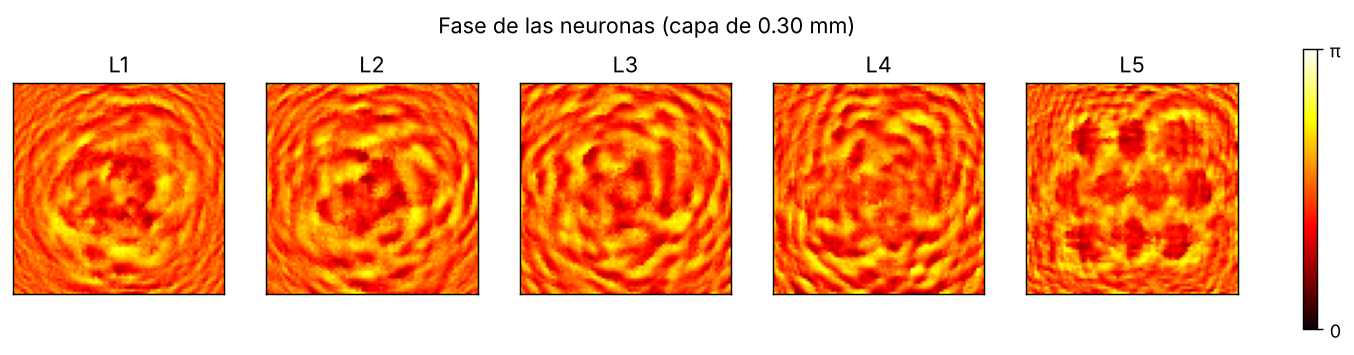
\includegraphics[width=0.70\textwidth]{fases.png}
\vspace{2pt}
\begin{columns}[T,onlytextwidth]
  \begin{column}{0.52\textwidth}
    \centering
    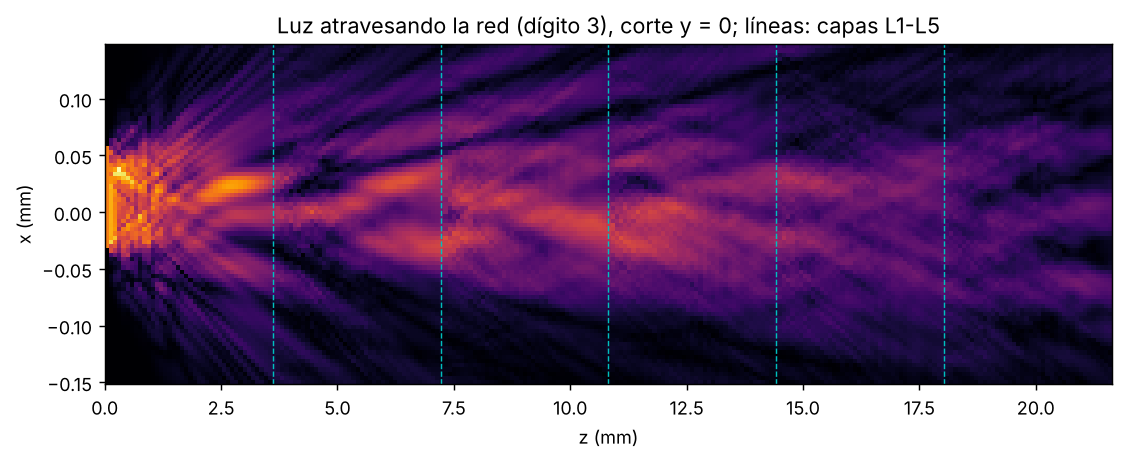
\includegraphics[width=0.83\textwidth]{corte_xz.png}\\[1pt]
    {\tiny Corte longitudinal $y=0$ (dígito 3): redistribución progresiva hasta enfocar el detector.}
  \end{column}
  \begin{column}{0.46\textwidth}
    \centering
    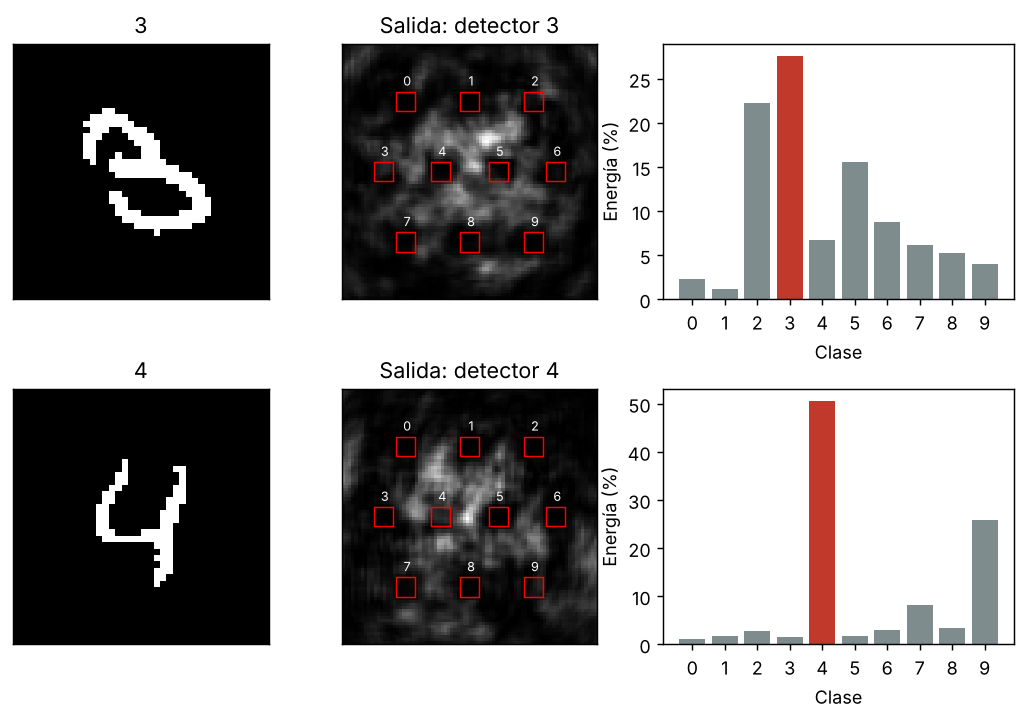
\includegraphics[width=0.75\textwidth]{fig3_ejemplos.png}\\[1pt]
    {\tiny Energía en los 10 detectores (arreglo 3--4--3): $L_5$ actúa como matriz de microlentes hacia cada caja.}
  \end{column}
\end{columns}
\end{frame}

% =====================================================================
%  DIAPOSITIVA 15: TOLERANCIAS DE FABRICACIÓN
% =====================================================================
\begin{frame}{Resultados IV: Tolerancias de fabricación ($91.6\% \to 84\%$)}
\framesubtitle{Evaluación del caso 2 (neurona \SI{3.8}{\micro m}) sin reentrenar bajo errores experimentales}
\centering
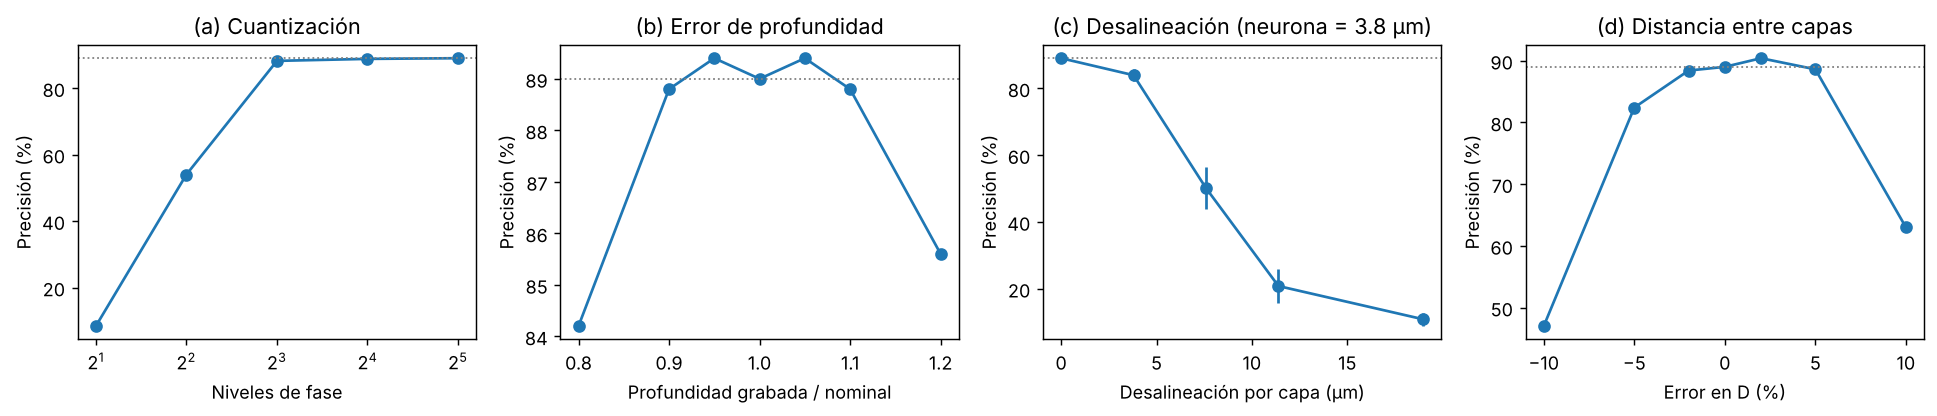
\includegraphics[width=0.84\textwidth]{fabricacion.png}
\vspace{2pt}
\begin{columns}[T,onlytextwidth]
  \begin{column}{0.32\textwidth}
    \begin{caja}{Cuantización litográfica}
      \scriptsize
      \begin{itemize}\setlength\itemsep{1pt}
        \item 2 niveles: 8.4\% \;\textbullet\; 4 niveles: 54.0\%
        \item \textbf{8 niveles (3 pasos): 88.2\%}
      \end{itemize}
      Justifica los 3 pasos litográficos.\\[1pt]
      \textbf{Eficiencia $\eta$:} sube $11\times$ ($1.6\%\to 18.6\%$) con $w=3$.
    \end{caja}
  \end{column}
  \begin{column}{0.32\textwidth}
    \begin{azulbox}{Profundidad y distancia $D$}
      \scriptsize
      \begin{itemize}\setlength\itemsep{1pt}
        \item Grabado $\pm 10\%$: $\ge 88.8\%$
        \item Distancia $\pm 5\%$: $\ge 82.4\%$
        \item Distancia $-10\%$: cae a 47.0\%
      \end{itemize}
    \end{azulbox}
  \end{column}
  \begin{column}{0.33\textwidth}
    \begin{destacado}
      \scriptsize
      \textbf{Desalineación lateral (crítica):}\\
      1 neurona (\SI{3.8}{\micro m}): \textbf{83.9\%}\\
      2 neuronas: 50.1\% \;\textbullet\; 3 neuronas: 20.8\%\\[1pt]
      \emph{Explica la caída experimental (84\%) del paper.}
    \end{destacado}
  \end{column}
\end{columns}
\end{frame}

% =====================================================================
%  DIAPOSITIVA 16: SISTEMA COMPLETO 1000x1000 (11 CLASES)
% =====================================================================
\begin{frame}{Resultados V: Sistema completo ($1000\times 1000$ neuronas, 11 clases)}
\framesubtitle{Reproducción en GPU (RTX~5060~Ti, \SI{16}{GiB}): \num{80000} imgs.\ entrenamiento, 6 épocas (\num{20004} pasos de Adam)}
\begin{columns}[T,onlytextwidth]
  \begin{column}{0.41\textwidth}
    \centering
    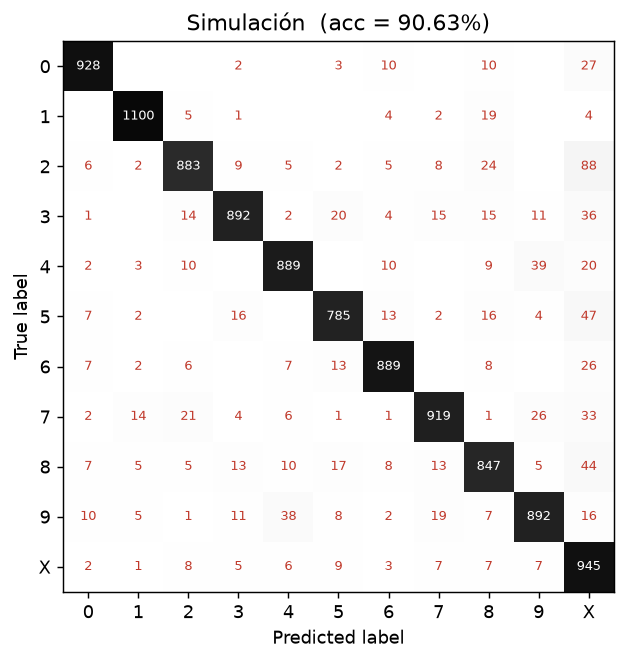
\includegraphics[width=0.92\textwidth]{full_confusion.png}\\[2pt]
    {\tiny Precisión total (\num{11000} imgs.): \textbf{90.63\%} (paper: 91.57\%)\\
    Dígitos 0--9: \textbf{90.24\%} \;\textbullet\; Clase X: \textbf{94.50\%}}
  \end{column}
  \begin{column}{0.57\textwidth}
    \centering
    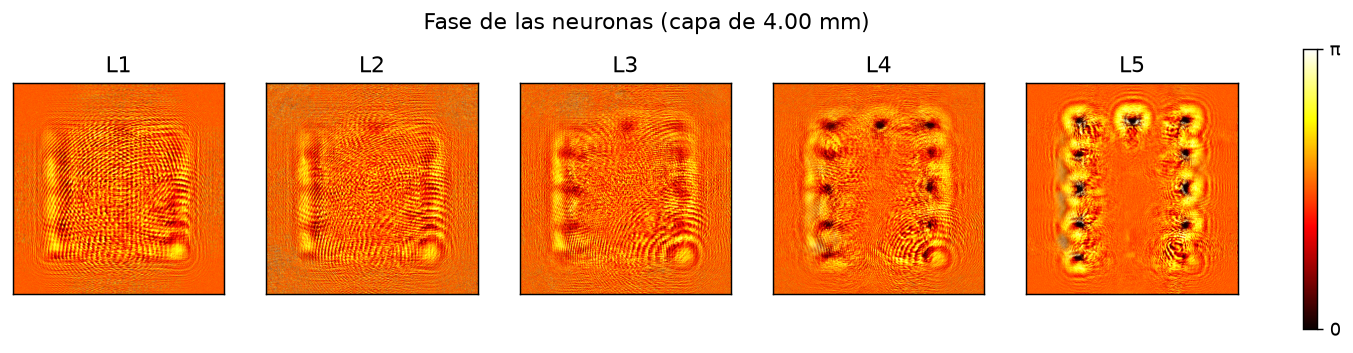
\includegraphics[width=\textwidth]{full_fases.png}\\[3pt]
    \begin{columns}[T,onlytextwidth]
      \begin{column}{0.49\textwidth}
        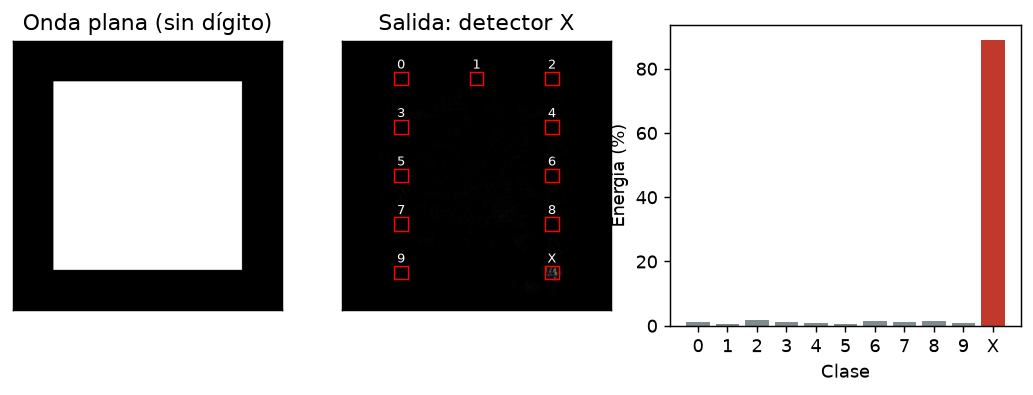
\includegraphics[width=\textwidth]{full_fig5_onda_plana.png}
      \end{column}
      \begin{column}{0.49\textwidth}
        \begin{destacado}
          \raggedright\scriptsize
          \textbf{Tiempo (RTX~5060~Ti, \texttt{--bs 24}):}\\
          \SI{20.32}{ms/img}, \SI{7.03}{GiB} VRAM; 6 épocas en \textbf{\SI{2.93}{h}} (\SI{29.3}{min}/época vs.\ $\approx\SI{1}{h}$/época en GTX~1080).\\[3pt]
          \textbf{Onda plana $\to$ X ($\approx 89\%$):}\\
          Rechaza entradas sin dígito. En $1000^2$, 8 niveles dan \textbf{91.05\%}, 1 neurona da \textbf{81.4\%}, y $\pm 2\%$ en $D=\SI{50}{mm}$ cae a 12--15\% ($\Delta D/D \le 1/\sqrt{N} = 0.10\%$).
        \end{destacado}
      \end{column}
    \end{columns}
  \end{column}
\end{columns}
\end{frame}

% =====================================================================
%  DIAPOSITIVA 14: CONCLUSIONES
% =====================================================================
\begin{frame}{Conclusiones}
\framesubtitle{Cinco lecciones de óptica difractiva}
\vspace{2pt}
\small
\begin{enumerate}\setlength\itemsep{4pt}
  \item \textbf{Difracción escalar exacta:} el sistema opera en campo cercano ($N_F\approx 126$) y fuera de Fresnel ($\SI{2.4}{rad}$--$\SI{9.7}{rad}$ en $\rho^4$); requiere el propagador de espectro angular completo.
  \item \textbf{Muestreo $=$ física:} $\varphi_{\max}=\arcsin(\lambda/2d_f)$ proviene del teorema de muestreo de Shannon--Nyquist, y $\Dmin=z_c$ unifica la conectividad geométrica con el límite de banda de Matsushima--Shimobaba.
  \item \textbf{Escalamiento paraxial y capas:} $N_{F,n}=d_f^2/(\lambda D)$ colapsa las curvas; al variar $L\in\{1,3,5,8\}$, el umbral baja como $1/(L+1)$ (de 18.2\% a 75.2\% en $0.03\,\Dmin$).
  \item \textbf{Sistema completo ($1000^2$, 11 clases) y gradiente holográfico:} el gradiente por Wirtinger acuerda a $\num{4.49e-16}$ con \texttt{autograd}, y la red completa en GPU alcanza \textbf{90.63\%} en \SI{2.93}{h} (\textbf{94.50\%} en clase~X).
  \item \textbf{Fabricación:} 8 niveles de fase bastan (88.2\% en $80^2$ y 91.05\% en $1000^2$), mientras que la alineación sub-neurona (83.9\% y 81.4\% con 1 neurona) y la tolerancia axial $\Delta D/D \propto 1/\sqrt{N}$ (0.10\% en $1000^2$) dominan el montaje.
\end{enumerate}
\vspace{2pt}
\begin{center}
  {\footnotesize\color{gris} Código, resultados, tesina y presentación: \texttt{github.com/AngelGab3/Final\_Project\_Optics\_Difractive\_Neural\_Networks}}
\end{center}
\end{frame}

\end{document}
